\documentclass[12pt]{article}
\usepackage{graphicx}
\usepackage{placeins}
\usepackage{amsmath}


% acronyms for text or math mode
\newcommand {\ccast} {\mbox{\small CCAST}}
\newcommand {\cris} {\mbox{\small CrIS}}

\newcommand {\airs} {\mbox{\small AIRS}}
\newcommand {\iasi} {\mbox{\small IASI}}
\newcommand {\idps} {\mbox{\small IDPS}}
\newcommand {\nasa} {\mbox{\small NASA}}
\newcommand {\noaa} {\mbox{\small NOAA}}
\newcommand {\nstar} {\mbox{\small STAR}}
\newcommand {\umbc} {\mbox{\small UMBC}}
\newcommand {\uw}   {\mbox{\small UW}}

\newcommand {\fft}  {\mbox{\small FFT}}
\newcommand {\ifft} {\mbox{\small IFFT}}
\newcommand {\fir}  {\mbox{\small FIR}}
\newcommand {\fov}  {\mbox{\small FOV}}
\newcommand {\for}  {\mbox{\small FOR}}
\newcommand {\ict}  {\mbox{\small ICT}}
\newcommand {\ils}  {\mbox{\small ILS}}
\newcommand {\igm}  {\mbox{\small IGM}}
\newcommand {\opd}  {\mbox{\small OPD}}
\newcommand {\rms}  {\mbox{\small RMS}}
\newcommand {\zpd}  {\mbox{\small ZPD}}
\newcommand {\ppm}  {\mbox{\small PPM}}
\newcommand {\srf}  {\mbox{\small SRF}}
\newcommand {\sdr}  {\mbox{\small SDR}}

\newcommand {\ES} {\mbox{\small ES}}
\newcommand {\SP} {\mbox{\small SP}}
\newcommand {\IT} {\mbox{\small IT}}
\newcommand {\SA} {\mbox{\small SA}}

\newcommand {\ET} {\mbox{\small ET}}
\newcommand {\FT} {\mbox{\small FT}}

% abbreviations, mainly for math mode
\newcommand {\real} {\mbox{real}}
\newcommand {\imag} {\mbox{imag}}
\newcommand {\atan} {\mbox{atan}}
\newcommand {\obs}  {\mbox{obs}}
\newcommand {\calc} {\mbox{calc}}
\newcommand {\sinc} {\mbox{sinc}}
\newcommand {\psinc} {\mbox{psinc}}
\newcommand {\std} {\mbox{std}}

% symbols, for math mode only
\newcommand {\wnum} {\mbox{cm$^{-1}$}}
\newcommand {\lmax} {L_{\mbox{\tiny max}}}
\newcommand {\vmax} {V_{\mbox{\tiny max}}}

\newcommand {\tauobs} {\tau_{\mbox{\tiny obs}}}
\newcommand {\taucal} {\tau_{\mbox{\tiny calc}}}
\newcommand {\Vdc}  {V_{\mbox{\tiny DC}}}

\newcommand {\rIT} {r_{\mbox{\tiny\textsc{ict}}}}
\newcommand {\rES} {r_{\mbox{\tiny\textsc{es}}}}
\newcommand {\robs} {r_{\mbox{\tiny obs}}}

\newcommand {\rITobs} {r_{\mbox{\tiny\textsc{ict}}}^{\mbox{\tiny obs}}}
\newcommand {\rITcal} {r_{\mbox{\tiny\textsc{ict}}}^{\mbox{\tiny cal}}}

\newcommand {\ITmean} {\langle\mbox{\small IT}\rangle}
\newcommand {\SPmean} {\langle\mbox{\small SP}\rangle}



\title{Modeling CrIS Nonlinearity \\
\vspace{3mm}
{****} DRAFT {****} \\
}

\author{H.~E.~Motteler and L.~L.~Strow \\
  \\
  UMBC Atmospheric Spectroscopy Lab \\
  Joint Center for Earth Systems Technology \\
}

\date{\today}
\begin{document}

\maketitle

We consider the definition of reference truth for measurements made
with a Michelson interferometer, taking into account relatively
small (or possibly non-existant) effects such as filter position and
potential mathematical artifacts.  The immediate application is
defining reference truth and a corresponding calibration equation
for the for the {\cris} instrument.

\section{Michelson Interferometer}

\begin{figure}
  \centering
  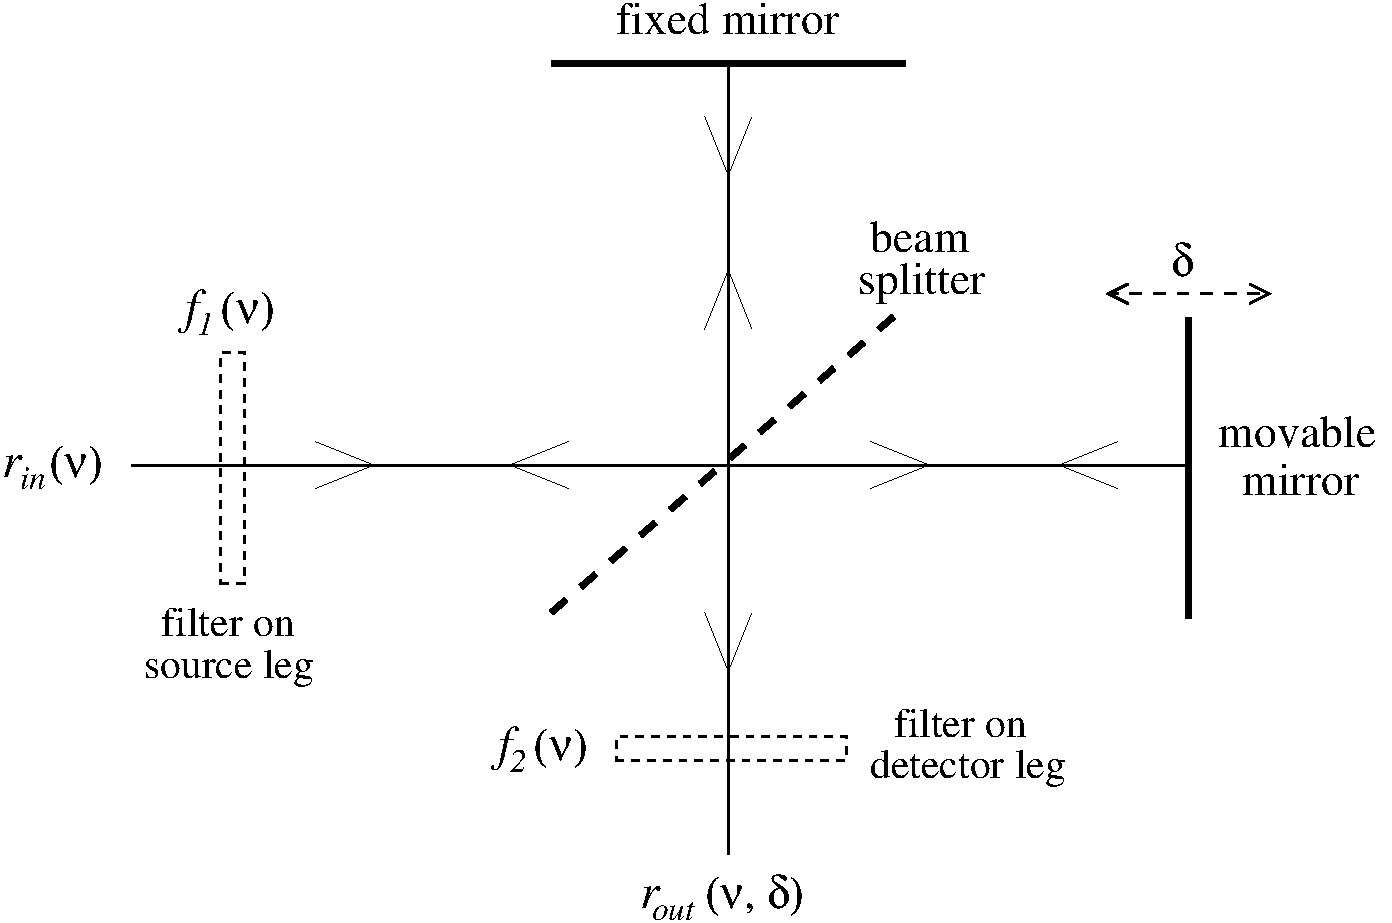
\includegraphics[scale=0.5]{figures/mich_filt2.pdf}
  \caption{Michelson interferometer with filters}
  \label{intf1}
\end{figure}

Figure \ref{intf1} shows a basic Michelson interferometer.  Let
$\rin(\nu)$ be incoming radiance as a function of frequency $\nu$,
$\delta$ mirror displacement, and $\rout(\nu, \delta)$ radiance on
the path to the detector.  In practice the signal from the detector
is the product of incoming radiance, beam-splitter efficiency, and
detector responsivity.  But suppose for the moment that we have a
perfect beam splitter and mirrors, and that there are no filters.
Then radiance $\rout$ on the path to the detector can be represented
as

\begin{equation}\label{eq1}
  \rout(\nu,\delta) = \rin(\nu)(1+\cos 2\pi\nu\delta)/2
\end{equation}

\noindent
including a term $\rin(\nu)/2$ that depends only on $\nu$.
Integrating over frequency, we have

\begin{equation}\label{eq2}
  \rout(\delta) = \frac{1}{2}\int_{\nu=0}^{\inf}\!\rin(\nu)d\nu + 
     \frac{1}{2}\int_{\nu=0}^{\inf}\!\rin(\nu)\cos(2\pi\nu\delta)d\nu
\end{equation}
\noindent
This is the continuous interferogram as a function of mirror
displacement~$\delta$.  We will want the consider the AC and DC
terms separately,

\begin{equation}\label{eq4}
  \rDC(\delta) =  \frac{1}{2}\int_{\nu=0}^{\inf}\rin(\nu)d\nu, \quad
  \rAC(\delta) =  \frac{1}{2}\int_{\nu=0}^{\inf}\rin(\nu)\cos(2\pi\nu\delta)d\nu
\end{equation}

$\rDC$ is a function of the scene, while $\rAC$ is a function of
both the scene and mirror position.  For $\delta = 0$ (zero mirror
displacement) the two terms are identical.

To measure $\rout(\delta)$ we might use a photodiode to convert
radiance to voltage.  Figure \ref{gainfun} shows sample transfer
functions for such a detector.  $G_1(r)$ and $G_2(r)$ are linear,
G(r) = br + c$, for some $b$ and $c$.  (For {\cris} $c$ is Vinst, a
DC bias value, while $b$ depends on analog gain and detector
properties.)  $G_3(r)$ is a hypothetical but plausible nonlinear
function.

Downstream from the the detector


[ transfer function should include photodiode and associated
  electronics ] 


\begin{figure}
  \centering
  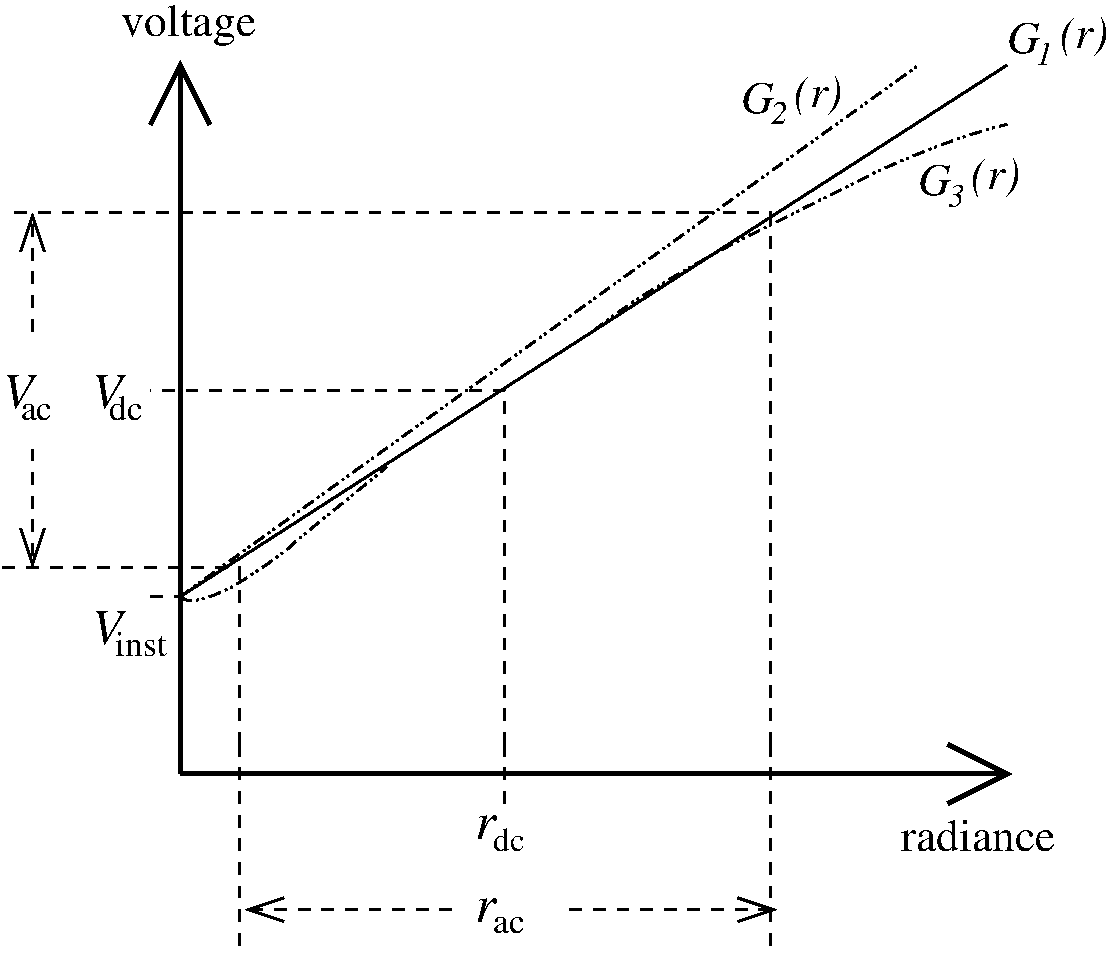
\includegraphics[scale=0.5]{figures/gain_fnx.pdf}
  \caption{typical transfer or gain functions}
  \label{gainfun}
\end{figure}

With {\cris}, we have a situation where there is observable
nonlinearlity or gain errors but the forward transfer function $G$
is not known explicitly.

Suppose $G(r) = ar^2 + br + c$







\end{document}

